\section{Implementation of the Lind Prototype}
\label{sec.implementation}

Based on the design introduced in Section \ref{sec.design},
we implemented a secure sandbox system, Lind,
for running untrusted user programs on vulnerable OS kernels.
Lind adapts two basic technologies as its building blocks\textendash
Google's Native Client (NaCl), and Seattle's Repy.

As described in Figure \ref{fig:design}, our design has
two main components\textendash a computation module that isolates the
application and a library OS module that isolates the complex
portions of POSIX.\lois{I don't believe POSIX has been introduced yet. Tell
the reader what it is.}
The Google's Native Client (NaCl) ~\cite{NaCl-09} served as the computation
module and Seattle's Repy as the library OS module (Figure \ref{fig:architecture}).\lois{Should
be a brief explanation of why you chose these particular components. There used to be
one in the past}

\begin{figure}%[h]
\centering
	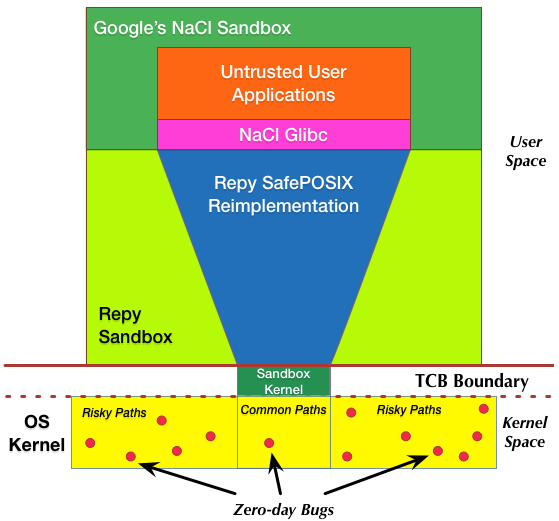
\includegraphics[width=1.0\columnwidth]{diagram/lind_architecture_new.png}
	\caption{Architecture of Lind including various components such as NaCl, NaCl glibc, and Repy Sandbox.
	User level application issues system calls that are dispatched through the Repy OS connector that bridges the Lind system to the OS Kernel.}

\label{fig:architecture}
\end{figure}

\subsection{The Computation Module of Lind: Google's Native Client}

We utilize NaCl in our design to isolate the computation of the user application
 from the kernel.
NaCl is a widely used environment for efficient execution of legacy code in the
form of x86 and ARM binaries, which allow Lind to work on most types of legacy code.
NaCl compiles the programs to produce a binary with software fault isolation.
This prevents the majority of the application from performing system calls
or executing arbitrary instructions.

To perform a system call, the application will call into a small privileged
part of the NaCl TCB that forwards system calls, usually to the OS or to Chrome for
processing \cappos{Check}.  To build Lind, we changed the NaCl TCP to
instead forward these calls to the SafePOSIX implementation
for processing. \lois{again, I don't think this terms was introduced} The NaCl
glibc module contains stubs that reject operations
that Chrome would not handle.  We added functionality to NaCl's glibc so that
those calls could be forwarded into SafePOSIX for processing.
\cappos{Need to compare NaCl execution w/ Chrome possibly
with fuzzing to others in the eval}


%NaCl can perform the functions required by the computation module well, and it is easy to
%connect with our system API module because NaCl uses glibc to perform system calls.
%Modification to NaCl's glibc would allow us to redirect those system call requests to our own system API module.
%
%NaCl is a sandbox used to execute untrusted x86 native code.
%It aims to give applications the computational performance of native applications without compromising safety.
%NaCl uses software fault isolation and a secure runtime to direct system interaction and
%side effects through interfaces managed by the program. It provides operating system portability
%for binary code while supporting performance-oriented features, such as thread support,
%instruction set extensions, such as SSE, and use of compiler intrinsics and a hand-coded assembler.
%It also allows the efficient execution of legacy code in the form of x86 and ARM binaries
%that are built with a lightly modified compiler tool chain.

\subsection{The Library OS Module of Lind: Seattle's Repy}

To build an API to access the safe parts of the underlying kernel, we need
two things.  First, we need a restricted sandbox that isolates computation
and only allows access to commonly used kernel paths.  We used
Seattle's Repy~\cite{Repy-10} sandbox to perform this task.
Second, we need to build a POSIX implementation to run within that sandbox.

%pplications. For Lind, we used Repy to build our system API module.
%To be more specific, our system API module has a very small sandbox kernel
%as TCB,  written with Python. On top of the sandbox kernel,
%we use Repy code to safely reimplement complex system functions.

\subsubsection{The Repy Sandbox Kernel}

As discussed earlier in Section \ref{sec.design}, the sandbox kernel needs to be secure and bug-free.
Because it is the TCB of the system, any bugs within it could cause fatal problems,
and allow attackers to access the OS kernel and gain kernel privilege.
We used Seattle's Repy system API module due to its tiny sandbox kernel
(comprised of only around 8,000 LOC)lois{is LOC always recognized ore should it be defined the
first time it appears?}. Using Repy also fit our key design principle that
our proposed system should only access the safe portions of the OS kernel.
The Repy sandbox kernel, has 33 basic API functions, including 13 network functions,
6 file functions, 6 threading functions,
and 8 miscellaneous functions
 (Table \ref{table:RepyKernel}) \cite{Repy-10}, \cite{RepyKernel}. Most of those functions are simple and
regularly used system calls that access the commonly used kernel paths.


\begin{table}
\centering
\caption {Repy sandbox kernel capabilities that supports NaCl functions, such as networking, file I/O operations and threading.}

  \begin{tabular}{ | p{2.5cm} | p{4.5cm} |}
  \hline
  \textbf{Repy Function} & \textbf{Available System Calls}  \\ \hline

Networking & \emph{gethostbyname, openconnection, getmyip, socket.send, socket.receive, socket.close,
listenforconnection, tcpserversocket.getconnection, tcpserversocket.close, sendmessage, listenformessage,
udpserversocket.getmessage, and udpserversocket.close.} \\ \hline

I/O Operations & \emph{openfile, file.close, file.readat, file.writeat, listfiles, and removefile.} \\ \hline

Threading & \emph{createlock, sleep, lock.acquire, lock.release, createthread, and getthreadname.} \\ \hline

Miscellaneous Functions & \emph{getruntime, randombytes, log, exitall, createvirtualnamespace,
virtualnamespace.evaluate, getresources, and getlasterror.}  \\ \hline
    \end{tabular}
    \label{table:RepyKernel}
\end{table}

%\begin{table}
%\centering
%\scriptsize
%\caption {System Functions in the Repy Sandbox Kernel.  \cappos{Need to
%clearly explain the takeaway.}}
%\begin{tabular}{|l|}
%  \hline
% \textbf{Network Functions} \\
%  \hline
%  gethostbyname(name) \\
%  \hline
%  getmyip() \\
%  \hline
%  openconnection(destip, destport, localip, localport, timeout) \\
%  \hline
%  socket.close() \\
%  \hline
%  socket.recv(numbytes) \\
%  \hline
%  socket.send(message) \\
%  \hline
%  listenforconnection(localip, localport) \\
%  \hline
%  tcpserversocket.getconnection() \\
%  \hline
%  tcpserversocket.close()\\
%  \hline
%  sendmessage(destip, destport, message, localip, localport) \\
%  \hline
%  listenformessage(localip, localport) \\
%  \hline
%  udpserversocket.getmessage() \\
%  \hline
%  udpserversocket.close() \\
%  \hline \hline
%  \textbf{File Functions} \\
%  \hline
%  openfile(filename, create) \\
%  \hline
%  file.close() \\
%  \hline
%  file.readat(sizelimit, offset) \\
%  \hline
% file.writeat(data, offset) \\
%  \hline
%  listfiles() \\
%  \hline
%  removefile(filename) \\
%  \hline \hline
%  \textbf{Threading Functions} \\
%  \hline
%  createlock() \\
%  \hline
%  lock.acquire(blocking) \\
%  \hline
%  lock.release() \\
%  \hline
%  createthread(function) \\
 % \hline
 % sleep(seconds) \\
  %\hline
  %getthreadname() \\
  %\hline \hline
  %\textbf{Miscellaneous Functions} \\
  %\hline
 % getruntime() \\
  %\hline
 % randombytes() \\
  %\hline
  %log(*args) \\
  %\hline
  %exitall() \\
  %\hline
  %createvirtualnamespace(code, name) \\
  %\hline
  %virtualnamespace.evaluate(context) \\
  %\hline
  %getresources() \\
  %\hline
  %getlasterror() \\
  %\hline
%\end{tabular}
%\label{table:RepyKernel}
%\end{table}

A natural concern with any sandbox design is that bugs are simply pushed into
another part of the trusted code base.  As it is the only piece of code added
to the system call paths of the TCB, the Repy sandbox kernel's security is of
paramount concern.

The sandbox kernel consists of only XXXX lines of code \cappos{continue...}.
The code is written to provide straightforward access to the minimal set
of the system call API needed to build general computational functionality.
The code is written using style guidelines designed to ease security auditing
 of the code~\cite{style}.

The sandbox kernel code has been
audited by a professional penetration tester.  Since 2010, there has also been
a bug bounty program for security flaws in the sandbox.
The code is deployed in daily use across thousands of devices,
including on the Seattle testbed \cite{seattle}, and has been examined by
hundreds of parties.  Developers have reported
XXX issues for problems in other parts of the systems. However, to date
no security flaws have been found in the sandbox kernel.
This does not provide any strong guarantees that bugs could not exist, and if
they do, the security of the system could be compromised.
However, having a small, easily auditable piece of code helps to reduce the
risk of this occurrence.

\subsubsection{The SafePOSIX Reimplementation}

The key responsibility of our system API module is to serve system call requests from user code.
In the Lind system, those system call requests are issued from the user code,
received by the computation module NaCl, and then redirected to our system API module.
The API module includes a POSIX API to serve those requests.

A POSIX API is a set of standard operating system interfaces that provide operating system functions
to the user code. However, the POSIX API is large and complex enough that its is
very hard to ensure that its implementation is secure and bug-free.\lois{Make sure this sentence
is correct. It was actually saying the opposite when I saw it yesterday. In discussion with
Yiwen I added the negative. But doublecheck.}

Our choice to use Repy helped us solve this architectural security problem.
Since Repy is a programming language sandbox, it can provide the ideal isolation
we needed when constructing our POSIX API. In Lind,
complex system functions are reimplemented using Repy code,
based on the ``safe-reimplement'' principle from our design in \S{\ref{sec.design}}.

\subsection{Operations}

Lind combines the NaCl and Repy components to provide native computation and
safe access to the system. Untrusted programs are run in NaCl,
but access to all system resources is diverted to a Repy program.
This program is responsible for accessing the system on behalf of the Lind library
 OS. A NaCl sandbox is built on top of the Repy sandbox.

To service a system call in NaCl, a server routine marshals its arguments into a text string,
and sends the call and the arguments to Repy sandbox.
The library OS then executes the appropriate system call, marshals the result and
returns it back to NaCl. The result is eventually returned as the appropriate native type to the calling program.

Lind is designed to minimize the need to modify either sandbox. This is possible
because the TCB of both were extremely small, and because the Lind code is run
in both\lois{Another odd sentence Yiwen and I discussed. I thought I knew how to
fix it, but it still does not make sense. I would delete it.}

The only complex part of Lind is the library OS, which runs in Repy.
However, because Python is a very powerful language that provides rich functions,
it significantly simplified the construction of Lind. \lois{I'm still not sure
how Python simplified contrusction}. Even though Python is considered ``slow'' by some,
the internals of an application in Lind are run in NaCl, a very high performance
environment. \lois{sentence above must be deleted or rephrased unless we can produce
evidence that Python is considered "slow."}
This balances the performance of the system, with the ease of implementation and maintenance
of the library OS component of Lind.

The novel idea behind the architecture and design for sandboxing using Lind
ensures the programs are portable.\lois{the "novel idea" is never spotlighted}
Programs running inside Lind are written to work against \lois{I don't think "against"
is the right word here} a standard POSIX glibc interface,
and, since the Lind runtime is strictly user-level, it can work on many different platforms
including Linux, Mac OS X and Windows.

The lightweight and minimized overhead is another feature of Lind. Because the sandbox only
 incurs overhead when there is a system call, overall overhead for Lind is low.
 Yet, it does not sacrifice performance for cost.
Lind uses a native interface for execution,
allowing CPU-and-memory-intensive applications to run at speeds that are equivalent
 to NaCl and near native speed.


In Sectioin \ref{sec.evaluation}}, we report how the dual sandboxes and other elements
of Lind performed in head-to-head evaluation against other virtualization systems.
